\chapter{VGMLの実装}\label{cha:Implementation}

本研究では、\ref{cha:Function}節で示した、既存手法の課題を解決するために、VDM++仕様書における以下の4つの構文を生成する手法を提案する。
さらに、提案手法を既存手法に適用し、機械学習を活用したVDM++仕様書自動生成ツールVGMLを開発する。

\begin{itemize}
    \item クラス
    \item インスタンス変数定義
    \item 関数定義
    \item 操作定義
\end{itemize}

本研究で開発するVGMLの構造を、図\ref{fig:vgml_structure}に示す。以降、4つの構文の生成手法について詳細を説明する。

\begin{figure}[t]
    \begin{center}
        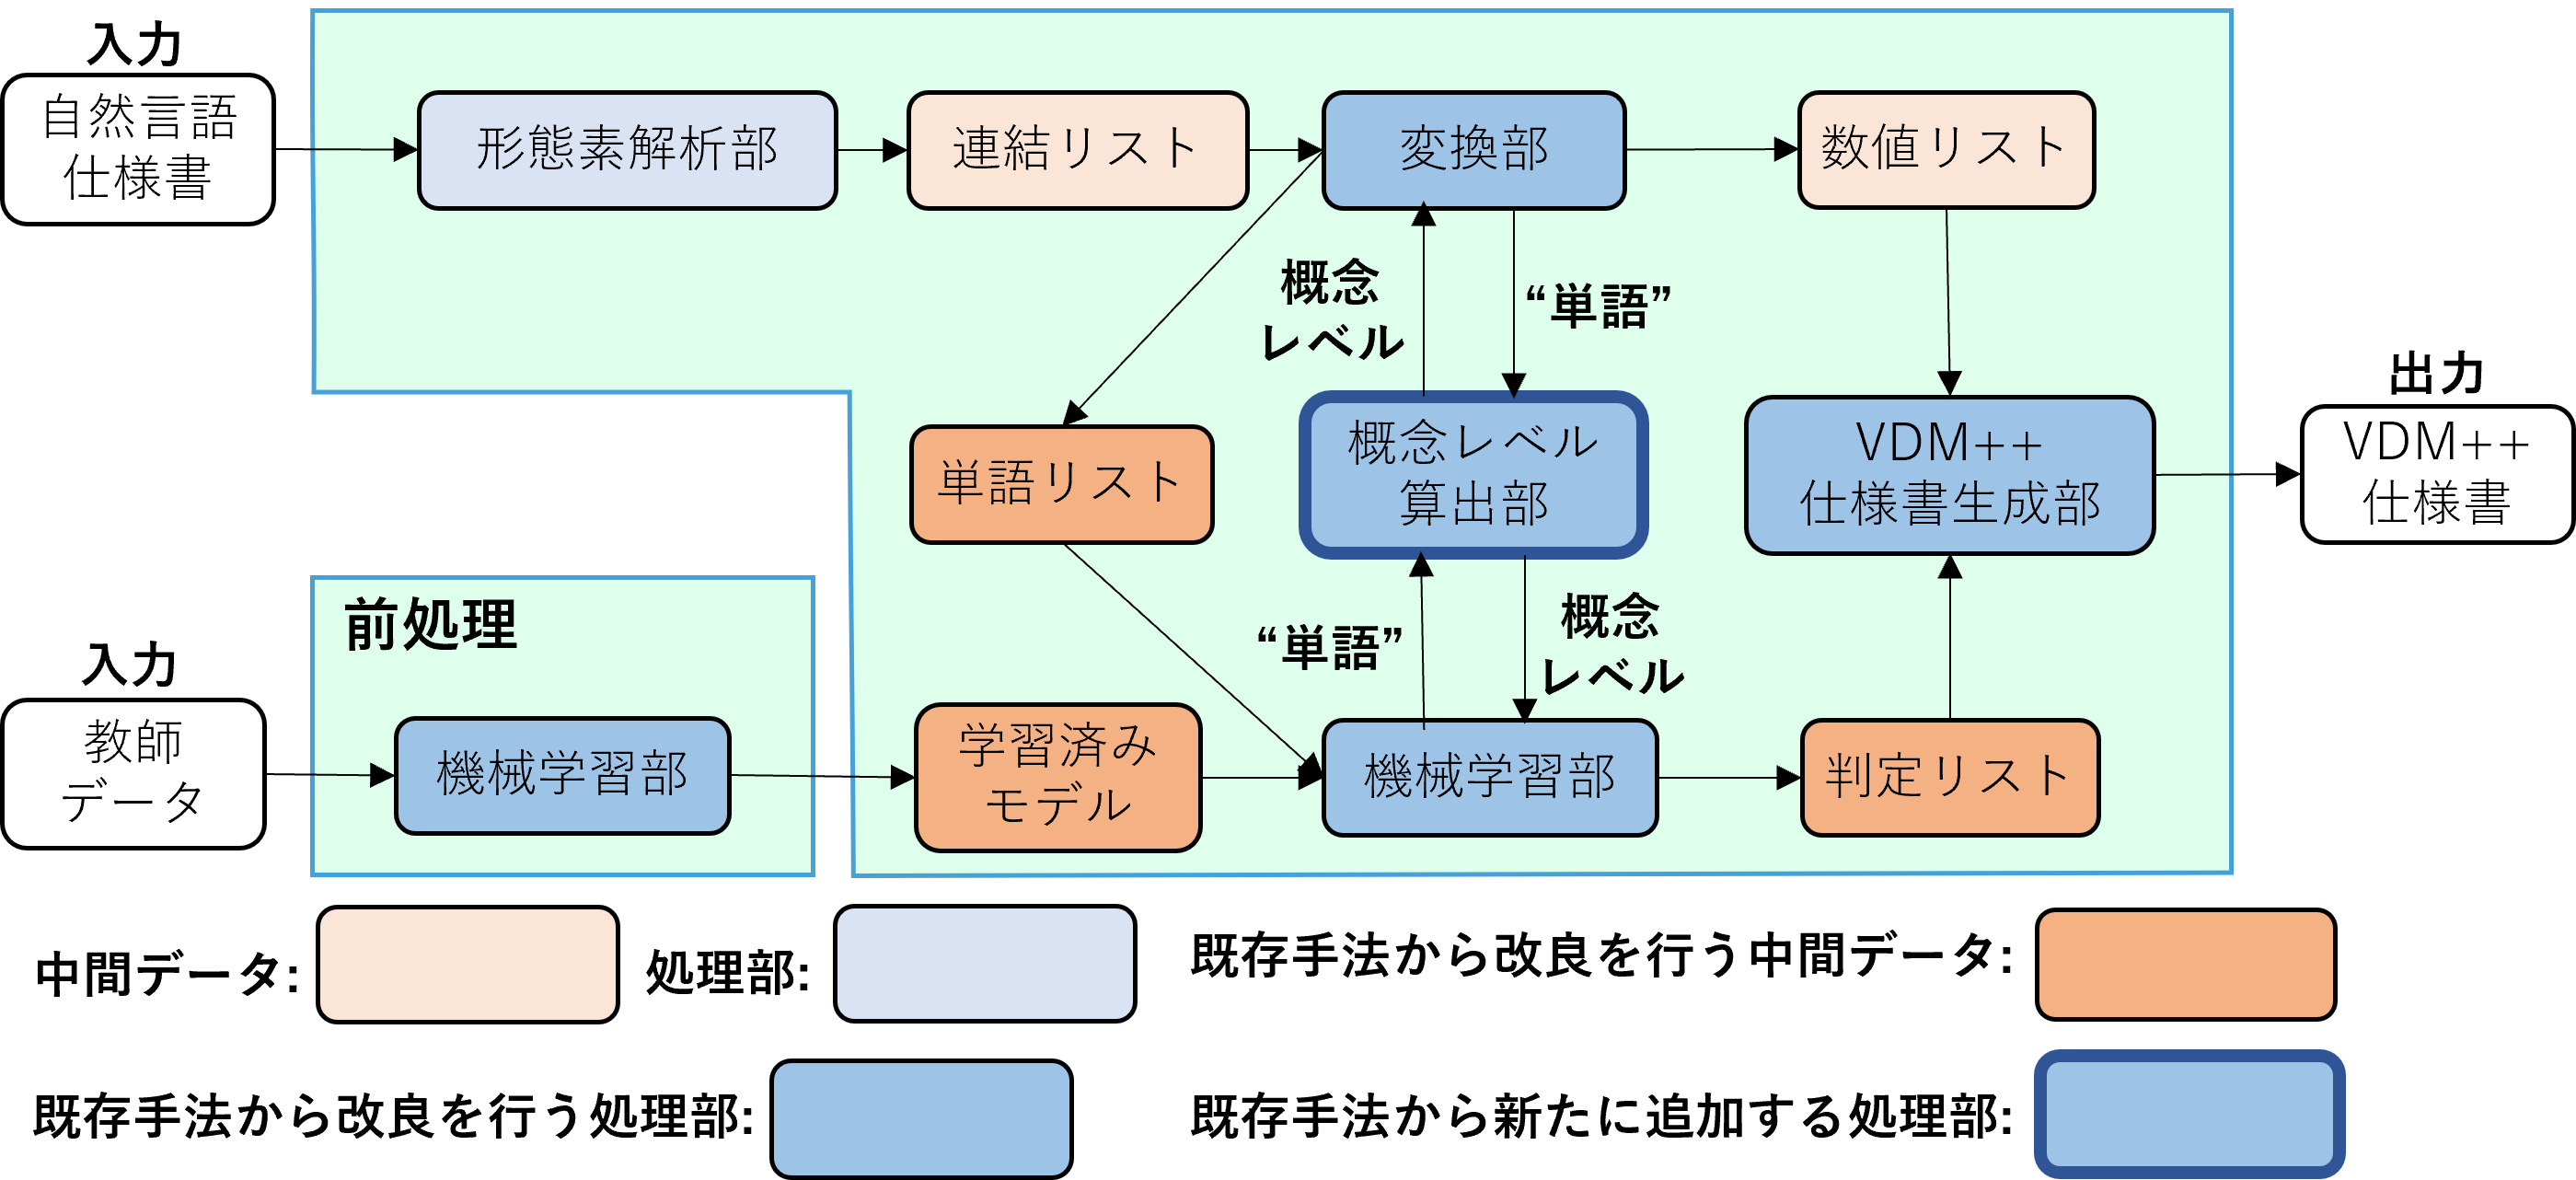
\includegraphics[width=1.0\columnwidth]{image/vgml_structure.png}
        \caption{VGMLの構造}
        \label{fig:vgml_structure}
    \end{center}
\end{figure}

\section{クラスへの対応}
本節では、自然言語仕様書からVDM++仕様書におけるクラスを生成する手法を提案する。具体的には、既存手法に対して以下の処理部の追加と改良を行う。

\begin{itemize}
    \item 各単語に対し本論文で新たに定義する概念レベルの算出処理部の追加。
    \item 変換部の自然言語仕様書内の単語にパラメータを追加する処理の改良。
    \item 機械学習部の学習済みモデルを生成する処理の改良。
    \item 機械学習部の自然言語仕様書内の単語を分類する処理の改良。
\end{itemize}

以降、4つの追加および改良した処理部について詳細を述べる。

\subsection{概念レベルの算出処理部の追加}
\label{sec:part_calc_concept_level}
既存手法は、機械学習に必要なパラメータとして、各単語に\ref{}節で述べたTF-IDF値、出現回数、優先値、連結回数の4つの値を追加する。
これにより、機械学習によって自然言語内の単語を、VDM++仕様書に必要である単語と、必要でない単語に分類することができる。

VGMLは、機械学習に必要なパラメータとして、各単語にTF-IDF値、出現回数、優先値、連結回数に加えて、本論文で新たに定義する概念レベルと合わせて5つの値を追加する(\ref{sec:improve_word_list}節に後述)。
これにより、機械学習によって自然言語仕様書内の単語を、VDM++仕様書に必要でない単語、VDM++仕様書に必要であるが、クラスの候補ではない単語、
VDM++仕様書に必要であり、かつ、クラスの候補である単語の3つに分類することができる。

概念レベルの計算は、\ref{}で述べた日本語WordNetを用いて、解析対象である単語とその下位概念の関係を表す木構造を生成する。
単語の下位概念の関係を表す木構造の例を、図\ref{}に示す。図\ref{}は、"りんご"の文字列を入力した際の木構造の例である。
日本語WordNetは、日本語での入力に対応しているが、出力する概念を表す単語は英語表記であるため、木構造を構成する単語も英語表記となる。
図\ref{}の木構造の場合、りんごの概念を持つ単語を最上位のノードとし、その下位概念である単語を子ノードとして表現する。
概念レベル算出部の構造を、図\ref{fig:vgml_concept_level_structure}に示す。概念レベル算出部は、1つの単語を入力として読み込み、算出した概念レベルを返す。
概念レベル算出部の処理の流れの例を図\ref{fig:flow_calc_concept_level}に、概念レベル算出部の処理の流れの説明を以下にそれぞれ示す。

\begin{figure}[t]
    \begin{center}
        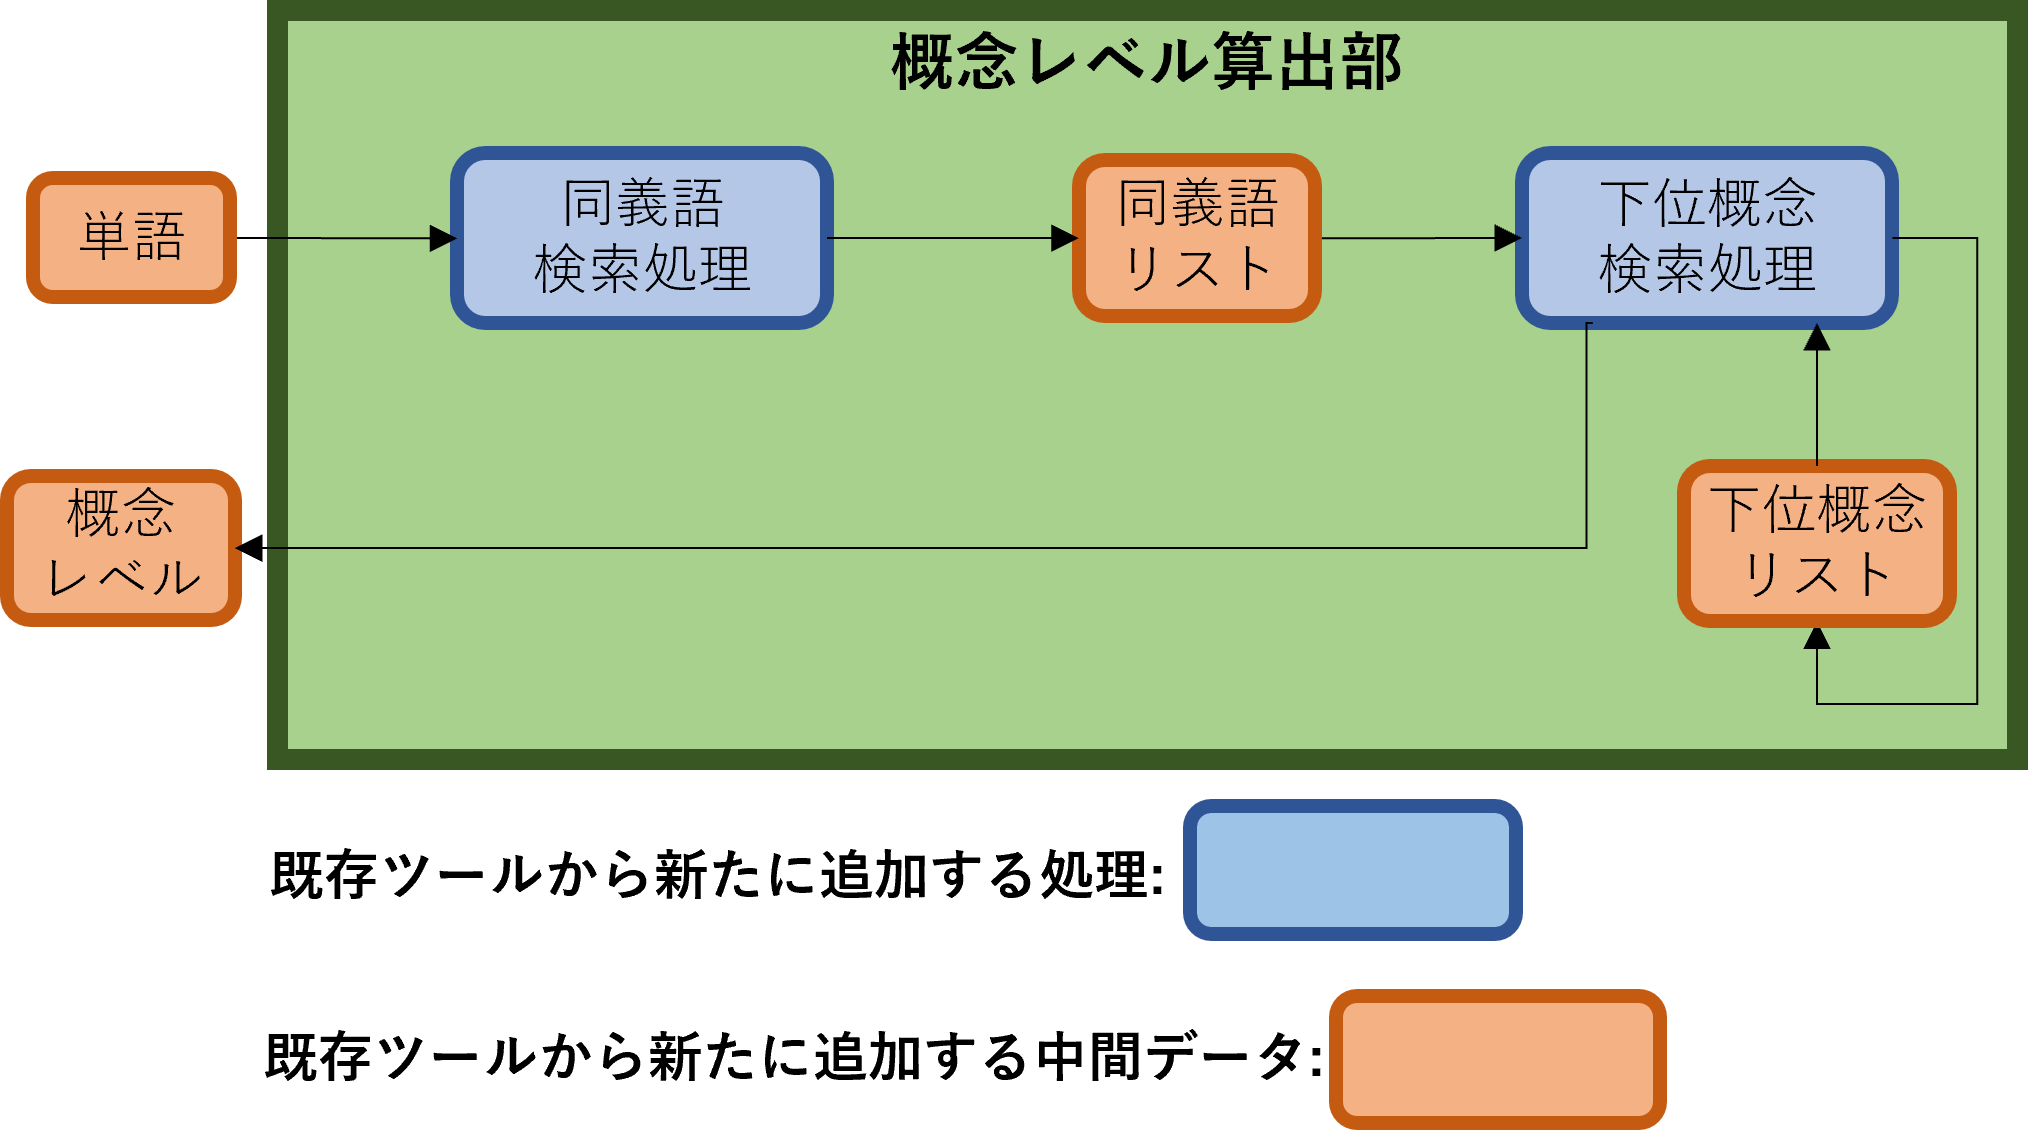
\includegraphics[width=1.0\columnwidth]{image/vgml_concept_level_structure.png}
        \caption{概念レベル算出部の構造}
        \label{fig:vgml_concept_level_structure}
    \end{center}
\end{figure}

\begin{figure}[t]
    \begin{center}
        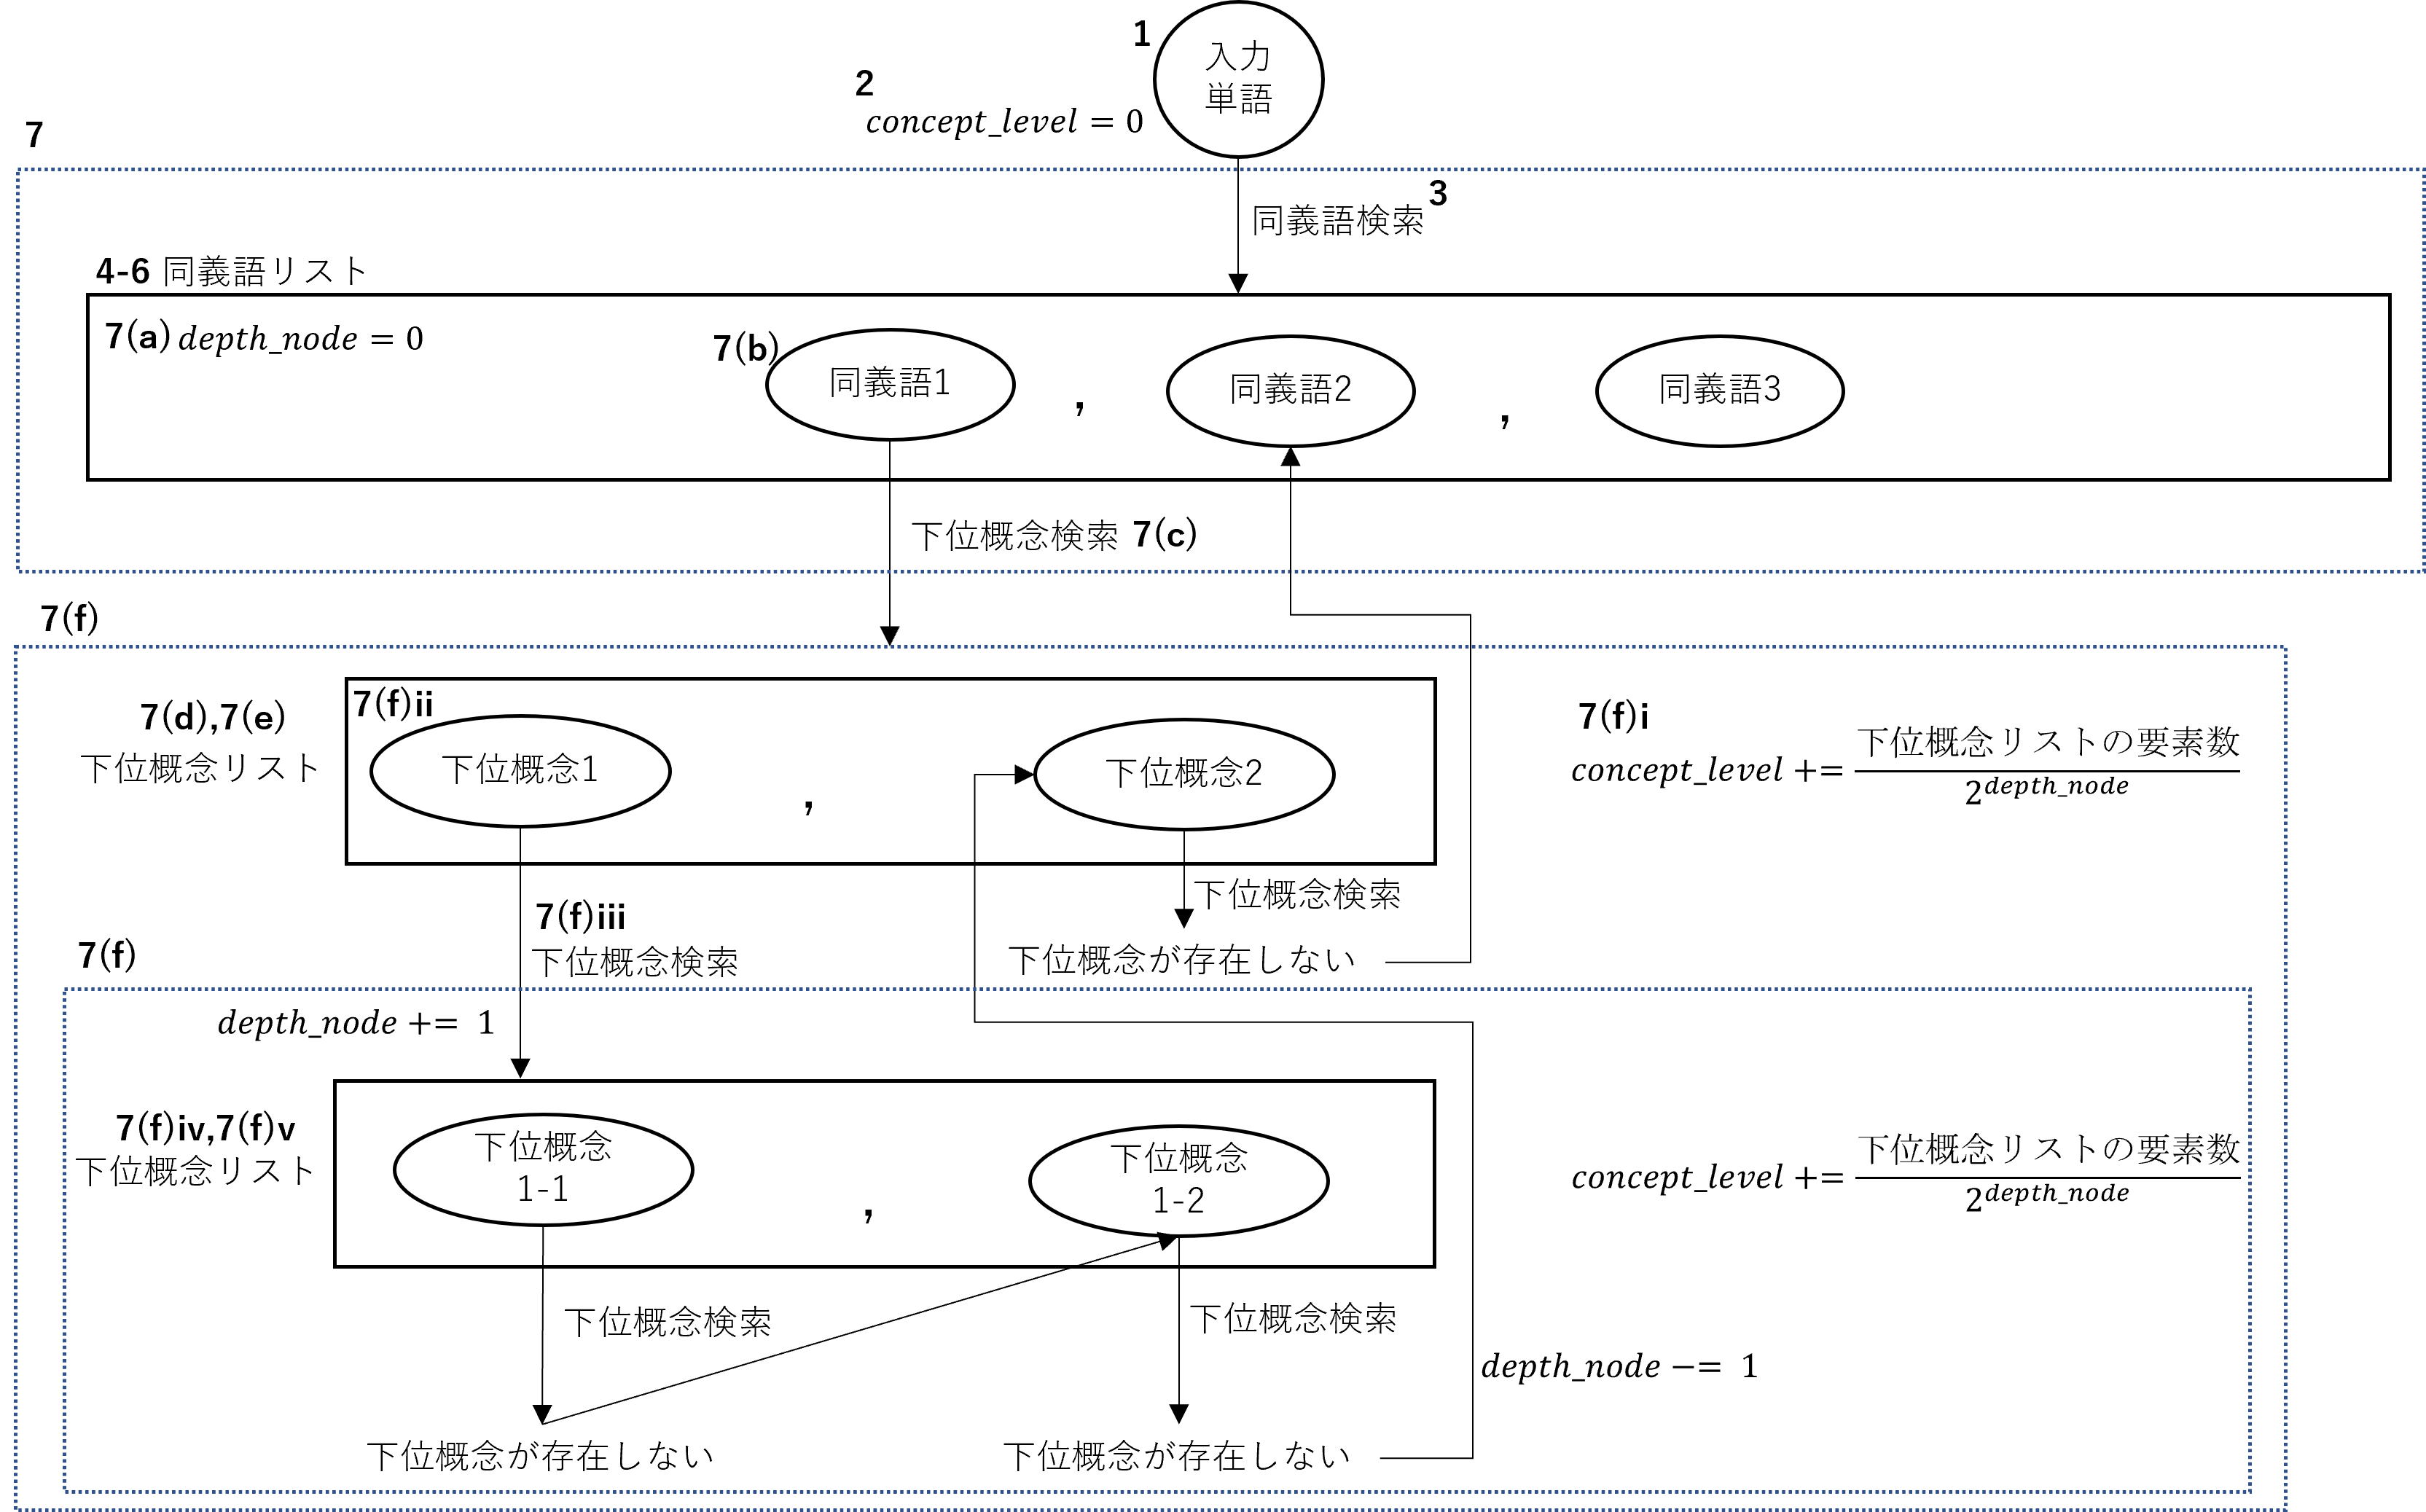
\includegraphics[width=1.0\columnwidth]{image/flow_calc_concept_level.png}
        \caption{概念レベル算出部の処理の流れの例}
        \label{fig:flow_calc_concept_level}
    \end{center}
\end{figure}

\begin{enumerate}
    \item 同義語検索処理は、単語を入力として読み込む。
    \label{sec:input_word}
    \item 同義語検索処理は、変数$concept\_level$を、0を初期値として定義する。変数$concept\_level$は、概念レベルを表す。
    \item 同義語検索処理は、日本語WordNetから\ref{sec:input_word}で入力した単語の同義語を検索する。
    \item 同義語検索処理は、空のリストを用意する。
    \label{sec:synonym_list}
    \item 検索した同義語を\ref{sec:synonym_list}で用意した空のリストに格納する。このリストを、以降、同義語リストと表現する。同義語が存在しない場合、概念レベルを0として返して処理を終了する。
    \item 同義語検索処理は、同義語リストを下位概念検索処理に渡す。
    \item 下位概念検索処理は、同義語リストの要素の数だけ以下の処理を繰り返す。
    \label{sec:loop_synonym_list}
        \begin{enumerate}
            \item 変数$depth\_node$を、0を初期値として定義する。変数$depth\_node$は、単語の上位下位の関係を表す木構造における、ノードの深さを表す。
            \item 同義語リストから、同義語を表す単語を1つ読み込む。
            \label{sec:read_synonym_word}
            \item 日本語WordNetから\ref{sec:read_synonym_word}で読み込んだ単語の下位概念を検索する。
            \item 空のリストを用意する。
            \label{sec:lower_concept_list}
            \item 検索した下位概念を\ref{sec:lower_concept_list}で用意した空のリストに格納する。このリストを、以降、下位概念リストと表現する。下位概念が存在しない場合、\ref{sec:loop_synonym_list}に戻る。
            \item 下位概念リストの要素の数だけ以下の処理を再帰的に繰り返す。
            \label{sec:loop_lower_list}
                \begin{enumerate}
                    \item $concept\_level$に$(下位概念リストの要素数\quad/\quad2^{depth\_node})$の値を加える。
                    \item 下位概念リストから、下位概念を表す単語を1つ読み込む
                    \label{sec:read_lower_word}
                    \item 日本語WordNetから\ref{sec:read_lower_word}で読み込んだ単語の下位概念を検索する。
                    \item 空のリストを用意する
                    \label{sec:lower_concept_list2}
                    \item 検索した下位概念を\ref{sec:lower_concept_list2}で用意した空のリストに格納する。
                    \label{sec:update_lower_concept_list}
                    \item \ref{sec:update_lower_concept_list}のリストに対し以下のいずれかの処理を行う。
                    \begin{itemize}
                        \item \ref{sec:update_lower_concept_list}のリストが空ではない、つまり、下位概念が存在する場合、\ref{sec:update_lower_concept_list}のリストを下位概念リストとし、$depth\_node$に1を加えて\ref{sec:loop_lower_list}に戻る。
                        \item \ref{sec:update_lower_concept_list}のリストが空である、つまり、下位概念が存在しない場合、\ref{sec:loop_lower_list}に戻る。
                        \item \ref{sec:update_lower_concept_list}のリストが空である、つまり、下位概念が存在しない、かつ、\ref{sec:read_lower_word}で読み込んだ単語が下位概念リストの末尾の要素である場合、$depth\_node$から1を引いて\ref{sec:loop_lower_list}に戻る。
                    \end{itemize}
                \end{enumerate}
        \end{enumerate}
\end{enumerate}

\subsection{自然言語仕様書内の単語にパラメータを追加する処理の改良}
\label{sec:improve_word_list}
既存手法は、図\ref{}に示す変換部において、各単語にTF-IDF値、出現回数、優先値、連結回数の4つの値を追加する。
さらに、図\ref{}に示す単語リストを生成する。
既存手法が生成する単語リストは、単語名と、各単語に対して算出した、TF-IDF値、出現回数、優先値、連結回数の4つのパラメータを持つ。

VGMLの変換部の構造を図\ref{fig:vgml_transfer}に、VGMLが生成する単語リストを図\ref{}にそれぞれ示す。
VGMLは、\ref{sec:part_fig:flow_calc_concept_level}節で述べた様に、図\ref{fig:vgml_concept_level_structure}に示す概念レベル算出部において、本論文で新たに定義する概念レベルを計算する。
さらに、変換部の概念レベル生成処理において、各単語に新たなパラメータとして概念レベルを追加し、図\ref{}に示す単語リストを生成する。
VGMLが生成する単語リストは、単語名と、各単語に対して算出した、TF-IDF値、出現回数、優先値、連結回数、概念レベルの5つのパラメータを持つ。

以降、VGMLの変換部における概念レベル生成処理の詳細について説明する。

\begin{enumerate}
    \item 連結回数生成処理より、図\ref{}
    \item 
\end{enumerate}


\begin{figure}[t]
    \begin{center}
        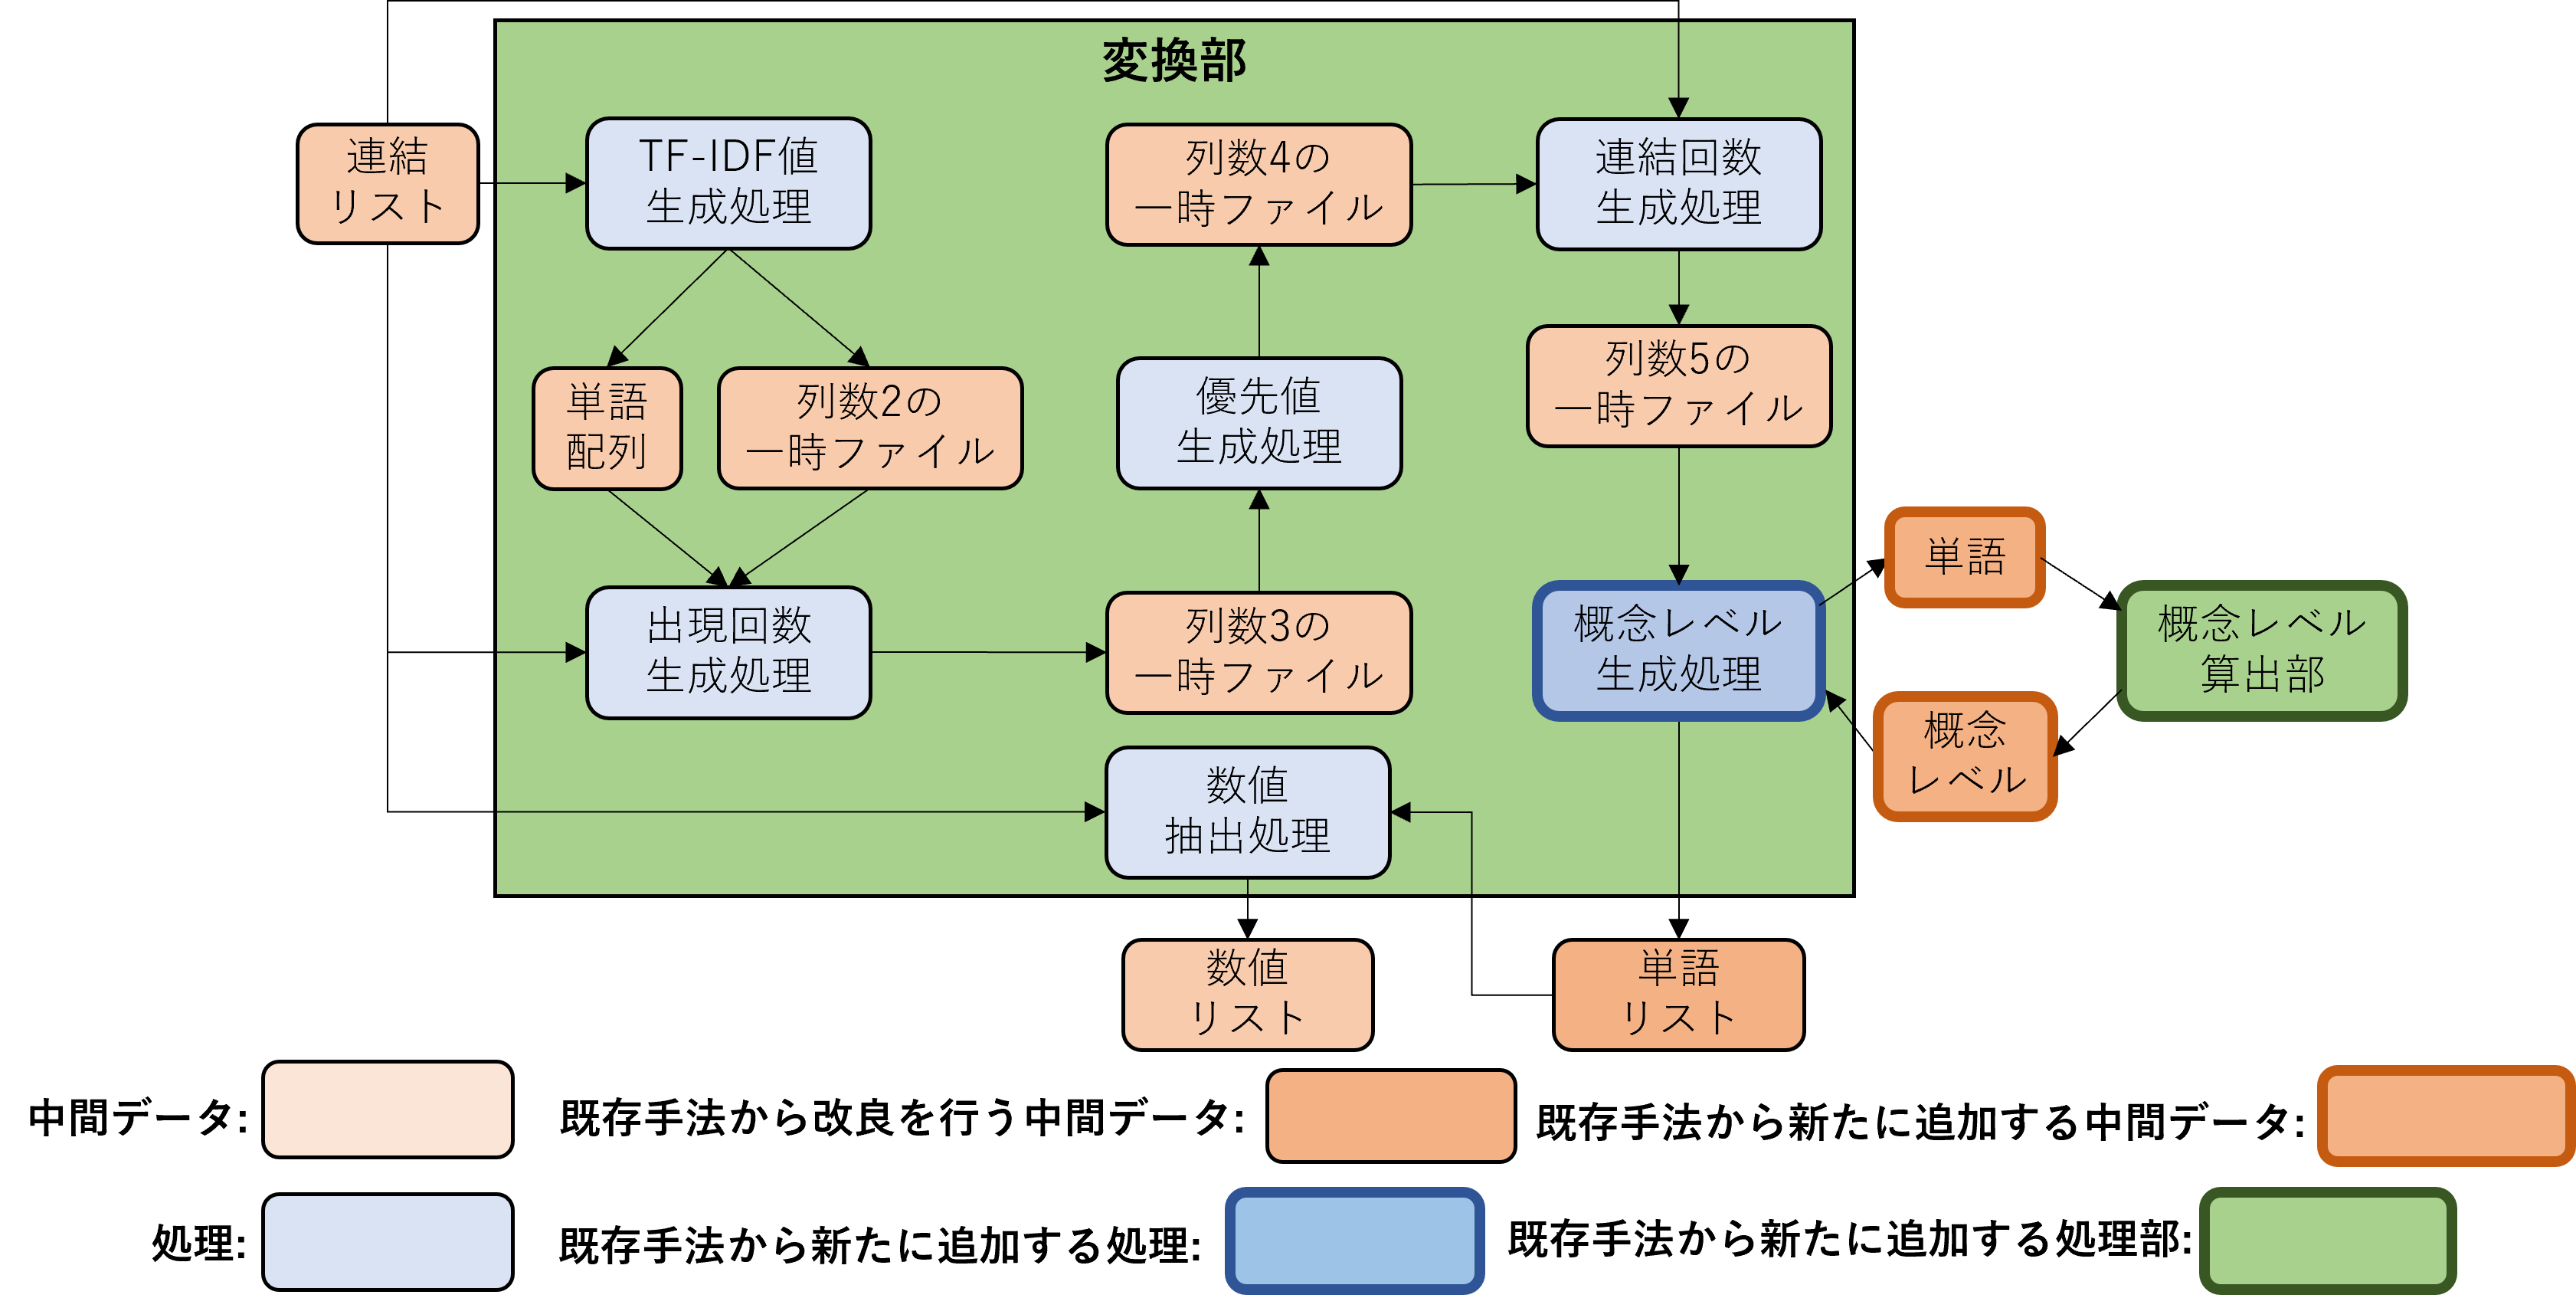
\includegraphics[width=1.0\columnwidth]{image/vgml_transfer.png}
        \caption{VGMLの変換部の構造}
        \label{fig:vgml_transfer}
    \end{center}
\end{figure}